\documentclass[tikz,border=5mm]{standalone}
\usepackage{tikz}
\usetikzlibrary{arrows.meta}

\begin{document}
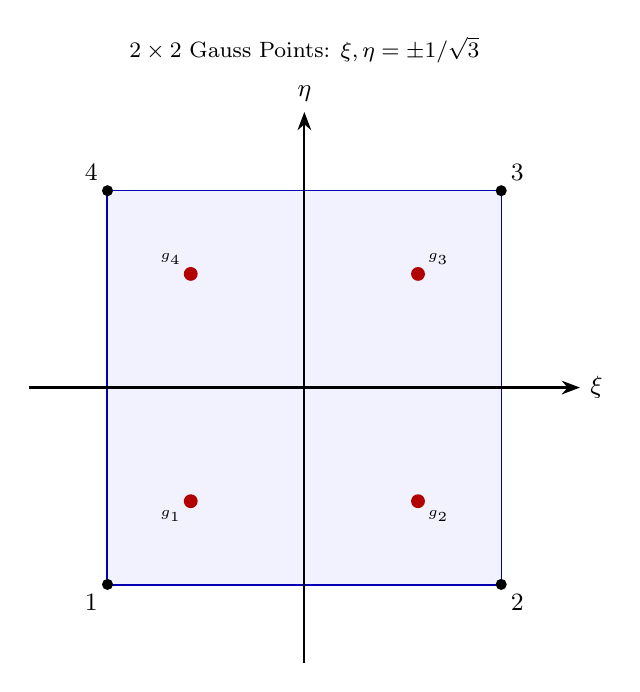
\begin{tikzpicture}[
    scale=2.5,
    gauss pt/.style={circle,fill=red!70!black,inner sep=0pt,minimum size=5pt},
    corner/.style={circle,fill=black,inner sep=0pt,minimum size=4pt}
]

\draw[thick,blue!70!black] (-1,-1) rectangle (1,1);
\fill[blue!5] (-1,-1) rectangle (1,1);

\pgfmathsetmacro{\g}{1/sqrt(3)}

\node[gauss pt] (g1) at (-\g,-\g) {};
\node[gauss pt] (g2) at (\g,-\g) {};
\node[gauss pt] (g3) at (\g,\g) {};
\node[gauss pt] (g4) at (-\g,\g) {};

\node[below left,font=\tiny] at (g1) {$g_1$};
\node[below right,font=\tiny] at (g2) {$g_2$};
\node[above right,font=\tiny] at (g3) {$g_3$};
\node[above left,font=\tiny] at (g4) {$g_4$};

\node[corner] at (-1,-1) {};
\node[corner] at (1,-1) {};
\node[corner] at (1,1) {};
\node[corner] at (-1,1) {};

\node[below left] at (-1,-1) {\small 1};
\node[below right] at (1,-1) {\small 2};
\node[above right] at (1,1) {\small 3};
\node[above left] at (-1,1) {\small 4};

\draw[-{Stealth},thick] (-1.4,0) -- (1.4,0) node[right] {\small $\xi$};
\draw[-{Stealth},thick] (0,-1.4) -- (0,1.4) node[above] {\small $\eta$};

\node[font=\footnotesize,anchor=south] at (0,1.6) {$2 \times 2$ Gauss Points: $\xi,\eta = \pm 1/\sqrt{3}$};

\end{tikzpicture}
\end{document}
